\documentclass[9pt,hyperref={unicode},utf8]{beamer}
\DeclareGraphicsRule{*}{mps}{*}{}
\usepackage{graphicx}
\usepackage{ifthen}
\usepackage{braket}
\usepackage{feynmp}
\usepackage{array}
\usepackage{calc}
\usepackage{fancybox}
\usepackage{xcolor}
\usepackage{feynmp}
\usepackage{color}
\usepackage{hepnames}
\usepackage{dcolumn}  % Align table columns on decimal point
\usepackage{amsmath}
\usepackage{bm}
\usepackage{multirow}
\usepackage{colortbl}
\usepackage{booktabs}
\usepackage{siunitx}
\usepackage{scrextend}
\usepackage{framed}
\usepackage[export]{adjustbox}
\definecolor{green}{rgb}{0.3,0.7,0.3}
\definecolor{blue}{rgb}{0.2,0.2,0.9}
\definecolor{red}{rgb}{0.9,0.2,0.2}
\definecolor{lightgray}{rgb}{0.4,0.4,0.4}
\newcommand\bbone{\ensuremath{\mathds{1}}}
\newcommand{\phione}{\ensuremath{\phi_{1}}}
\newcommand{\phitwo}{\ensuremath{\phi_{2}}}
\newcommand{\phionebeta}{\ensuremath{\phi_{1}(\beta)}}
\newcommand{\phitwoalpha}{\ensuremath{\phi_{2}(\alpha)}}
\newcommand{\ccs}{\ensuremath{\Pqb\to\Pqc\Paqc\Pqs}}
\newcommand{\dqq}{\ensuremath{\Pqb\to\Pqd\Pq\Paq}}
\newcommand{\uud}{\ensuremath{\Pqb\to\Pqu\Paqu\Pqd}}
\newcommand{\sqq}{\ensuremath{\Pqb\to\Pqs\Pq\Paq}}
\newcommand{\BsJpsiKK}{\ensuremath{\PBs\rightarrow \PJpsi\PK\PK} }
\newcommand{\KsPizMuMu}{\ensuremath{\PKzS\rightarrow \Pgpz\APmuon\Pmuon} }
\newcommand{\KsPipPim}{\ensuremath{\PKzS\rightarrow\Pgpp\Pgpm} }
\newcommand{\PBud}{\ensuremath{\PB_{ud}} }
\newcommand{\BBbar}{\ensuremath{\PB\PaB} }
\newcommand{\dt}{\ensuremath{\Delta t}}
\newcommand{\taub}{\ensuremath{\tau_{\PBz}}}
\newcommand{\Dmd}{\ensuremath{\Delta m_{d}}}
\newcommand{\mybox}[2]{{\color{#1}\fbox{\normalcolor#2}}}
\newcommand{\Acp}{\ensuremath{{\cal A}_{CP}}}
\newcommand{\Scp}{\ensuremath{{\cal S}_{CP}}}
\setlength{\fboxrule}{1pt}
% \newcommand{\APKst}{\HepParticle{\bar K^{\ast0}}{}{}}
\DeclareRobustCommand{\APKst}{\HepAntiParticle{K}{}{\ast0}\xspace}
\usetheme{Amsterdam}
\makeatletter
\setbeamertemplate{footline}
{
    \leavevmode%
    \hbox{%
        \begin{beamercolorbox}[wd=.333333\paperwidth,ht=2.25ex,dp=1ex,center]{author in head/foot}%
            \usebeamerfont{author in head/foot}\insertshortauthor
        \end{beamercolorbox}%
        \begin{beamercolorbox}[wd=.333333\paperwidth,ht=2.25ex,dp=1ex,center]{title in head/foot}%
            \usebeamerfont{title in head/foot}\insertshorttitle
        \end{beamercolorbox}%
        \begin{beamercolorbox}[wd=.333333\paperwidth,ht=2.25ex,dp=1ex,right]{date in head/foot}%
            \usebeamerfont{date in head/foot}\insertshortdate{}\hspace*{2em}
            \insertframenumber{}\hspace*{2ex}  %/ \inserttotalframenumber\hspace*{2ex} 
        \end{beamercolorbox}}%
        \vskip0pt%
    }
    \makeatother
\usepackage{tikz}
\usetikzlibrary{arrows,shapes,backgrounds}
\setbeamertemplate{title page}[noinstitute]
\setbeamertemplate{mini frames}{}
\renewcommand*{\slideentry}[6]{}

\AtBeginSection[]
{
  \begin{frame}
    \frametitle{Outline}
    \tableofcontents[currentsection]
  \end{frame}
}
\AtBeginSubsection[]
{
  \begin{frame}
    \frametitle{Outline}
    \tableofcontents[currentsection, currentsubsection]
  \end{frame}
}
\tikzset{
    myarrow/.style={
        draw,
        fill=red,
        single arrow,
        minimum height=80ex,
        maximum width=1ex,
        single arrow head extend=1ex
    }
}
\newcommand{\arrowup}{%
\tikz [baseline=0.1ex]{\node [myarrow,rotate=-170] {};}
}
\tikzstyle{every picture}+=[remember picture]
\tikzstyle{na} = [baseline=-.5ex]

\title[\KsPizMuMu]{\bf Sensitivity study of \texorpdfstring{\KsPizMuMu}{KS->pi0mu+mu-}}
\author[Veronika Chobanova]{\textbf{Veronika Chobanova, Diego Mart\'{i}nez Santos, Miriam Lucio Mart\'{i}nez}\\ University of Santiago de Compostela}
\date{9 September 2016}
\def\follows{$\Rightarrow$~}
\begin{document}

\begin{frame}
           
    \titlepage
    \begin{minipage}{0.69\textwidth}
      \includegraphics[height=28pt]{../figs/erc.pdf}
      \includegraphics[height=33pt]{../figs/usc.pdf}\\
      \includegraphics[height=23pt]{../figs/XuntaGalicia.jpg}\hspace{5.5cm}
    \end{minipage}
    \begin{minipage}{0.3\textwidth}
      \includegraphics[height=28pt,right]{../figs/lhcb.pdf}
    \end{minipage}
\end{frame}

\setbeamertemplate{sidebar right}[pagenum]
 
\begin{frame}{Physics motivation}
 \begin{minipage}{0.35\textwidth}
  \includegraphics[width=0.99\textwidth]{Cirigliano_fig17.pdf}
 \end{minipage}
 \begin{minipage}{0.64\textwidth}
  \begin{itemize}
  \setlength\itemsep{1.2em}
   \item $\PKz\to\Pgpz\APmuon\Pmuon$ is a very rare decay, strongly supressed in the SM
   \item $\Pqs\to\Pqd$ transitions potentially sensitive to NP, especially to new sources of flavor violation
  \end{itemize}
 \end{minipage}\\
 \vspace{0.5cm}
  \begin{itemize}
%   \setlength\itemsep{0.5em}
     \item $\textcolor{red}{\PKzL\to\Pgpz\APmuon\Pmuon}$ order of magnitude variation of the BR in models
     with Extra Dimensions,  \href{arXiv:0912.1625 [hep-ph]}{\underline{JHEP09(2010)017}}
     \item[]
     \item ${\cal B}(\textcolor{red}{\PKzL\to\Pgpz\APmuon\Pmuon})$ SM theory uncertainty large, $\approx 20\%$
     \item[] $\rightarrow$ Limited by experimental precision of
     \item[] \textcolor{white}{$\rightarrow$} ${\cal B}(\textcolor{green}{\PKzS\to\Pgpz\APmuon\Pmuon})=(2.9^{+1.5}_{-1.2}\text{(stat)}\pm0.2\text{(syst)})\times10^{-9}$,
     \href{https://cds.cern.ch/record/777240/files/phep-2004-025.pdf}{\underline{NA48 paper}}
     \item[]
     \item \textbf{Sensitivity study} -- LHCb precision of ${\cal B}(\textcolor{green}{\PKzS\to\Pgpz\APmuon\Pmuon})$ with future data
  \end{itemize}
\end{frame}


\begin{frame}{Event selection}
 \centering
   \begin{table}
    \textbf{\underline{Two separate analyses: FULL and PARTIAL}}\\
   \renewcommand{\arraystretch}{1.5}
   \begin{tabular}
       {l@{\hspace{0.7cm}}l@{\hspace{0.6cm}}l}\\
        \toprule
        & {\bf FULL} & {\bf PARTIAL} \\
        \midrule
        Reconstruction & $\Pgpz[\Pphoton\Pphoton]\APmuon\Pmuon$ & \parbox[t]{4cm}{Only $\APmuon\Pmuon$, artificial \Pgpz\ with $p_{z}(\Pgpz)\approx\SI{10}{\giga\eV}/c$ added\\ 
        $\rightarrow$ best $M_{\Pgpz\APmuon\Pmuon}$ resolution}\\
%         && \\
%         \Pgpz constraints & \multicolumn{2}{l}{\hspace{1.5cm}$M(\Pphoton\Pphoton) = m(\Pgpz)$}\\
%          & \multicolumn{2}{l}{\hspace{1.5cm}IP(\PKzS) = 0, constrains $p(\Pgpz)$}\\
%          & \multicolumn{2}{l}{\hspace{1.5cm}\Pgpz required to originate from SV}\\
%         && \\
        Data & Run I ($\SI{3}{\per\femto\barn}$) & 2016 ($\SI{0.3}{\per\femto\barn}$ ) \\
        Stripping & Stp21 & Stp26  \\
        Stripping line &K0s2Pi0MuMuLines & TriggerTestLine\\
        MC & 2012 & 2015  \\
%         Rec. and sel. efficiency & $5.5\times10^{-4}$  & $3.0\times10^{-3}$  \\
        \bottomrule
   \end{tabular}
 \end{table}
\end{frame}

\begin{frame}{Event selection}
 \textbf{Main stripping requirements}
 \vspace{0.2cm}
 \begin{itemize}
  \setlength\itemsep{0.8em}
  \item \Pmu: $p_{T}(\Pmu)>\SI{80}{\mega\eV}/c$, hits in VELO, TT, T-stations and muon chambers
  \item \Pphoton: $p_{T}(\Pphoton)>\SI{200}{\mega\eV}/c$, resolved (FULL only)
  \item \Pgpz: $|M_{\Pphoton\Pphoton}-m(\Pgpz)|<\SI{30}{\mega\eV}/c^{2}$ (FULL only)        
  \item[] \Pgpz constraints: $M(\Pphoton\Pphoton) = m(\Pgpz)$; IP(\PKzS) = 0, constrains $p(\Pgpz)$; \\ \hspace{2.1cm} \Pgpz required to originate from SV
  \item $\Pmu\Pmu$: $M_{\Pmu\Pmu} < \SI{450}{\mega\eV}/c^{2}$ (PARTIAL only)
  \item \PKzS: $400 < M_{\Pgpz\APmuon\Pmuon} < \SI{600}{\mega\eV}/c^{2}$
  \item[]
  \item $\epsilon_{\rm stp}(\rm FULL) = 1.8\times10^{-4}$\\ $\epsilon_{\rm stp}(\rm PARTIAL) = 1.2\times10^{-3}$
 \end{itemize}
\end{frame}
 
\begin{frame}{Event selection}
  \textbf{Fiducial cuts}
 \vspace{0.2cm}	
  \begin{itemize}
  \setlength\itemsep{0.8em}
    \item $\tau_{\PKzS}>\SI{1}{\pico\s}$
    \item Hits in TT $>0.1$ for both muons
    \item ProbNN $>0.05$
    \item $M_{\Pgpz\APmuon\Pmuon} < \SI{490}{\mega\eV}/c^{2}$
    \item Kinematic cut to remove $\Lambda\to\Pp\Pgp$, $\PKzS\to\Pgpp\Pgpm$ (Armenteros-Podolanski)
  \end{itemize}
  
  \vspace{0.5cm}
  
  \centering
  \begin{minipage}{0.5\textwidth}
    \begin{framed}
    $\epsilon_{\rm tot} = \epsilon_{\rm gen}\times\epsilon_{\rm stp}\times\epsilon_{\rm fid}$\\
    $\epsilon_{\rm tot}(\rm FULL) = 5.5\times10^{-4}$\\
    $\epsilon_{\rm tot}(\rm PARTIAL) = 3\times10^{-3}$
    \end{framed}
  \end{minipage}
\end{frame}


\begin{frame}{MVA}
 \begin{itemize}
  \setlength\itemsep{0.3em}
%   \item Fit to the reconstructed \PKzS candidate mass in bins of MVA 
  \item Major background: combinatorial, suppressed with an MVA
  \item FULL and PARTIAL treated separately in training and fitting
  \item[] $\rightarrow$ MC for signal
  \item[] $\rightarrow$ Data for combinatorial background (TIS at all trigger levels)
  \item[] \textcolor{white}{$\rightarrow$} Data for training not used in the fit to the data
 \end{itemize}
 \end{frame}
\begin{frame}{MVA}
 \centering
 \textcolor{red}{\bf MVA training in three steps}\\
 
 \vspace{0.2cm}
 
  \textcolor{red}{{\bf Step 1} Continuous variables gaussianized, decorrelated and gaussianized again} \\
  
  \vspace{0.3cm}
  %(geometrical\\ likelihood)
 \begin{minipage}{0.45\textwidth}
    \begin{itemize}
     \setlength\itemsep{0.7em}
      \item \PKzS: IPs, $p_{T}$, vertex $\chi^{2}$, flight distance significance
      \item \Pmu: track fit $\chi^{2}$/NDF\textcolor{blue}{$^1$}, IPs, PID\textcolor{blue}{$^2$}, DOCA ($\APmuon\Pmuon$)
      \item Angle between $\Pmu\Pmu$ and $\Pphoton\Pphoton$ planes (FULL only)
    \end{itemize}
    
  \begin{itemize}
  \setlength\itemsep{0.7em}
    \item $M(\Pphoton\Pphoton)$\textcolor{blue}{$^3$} (FULL only)
    \item Helicity angles (FULL only)
    \item SV coordinates\textcolor{blue}{$^4$} (suppress material interactions)
  \end{itemize}
 \end{minipage}
 \begin{minipage}{0.54\textwidth}
    
    \vspace{1cm}
%     \hspace{0.5cm} \textcolor{red}{---} signal \hspace{0.5cm} {---} background\\
    \includegraphics[width=0.49\textwidth]{mu1_track_Chi2DoFFULL.pdf}
      \put(-65,43){\textcolor{blue}{$1$}}
     \put(-25,42){\footnotesize{FULL}}
    \includegraphics[width=0.49\textwidth]{PIDmu1PARTIAL.pdf}
      \put(-65,43){\textcolor{blue}{$2$}}
      \put(-67,13){\footnotesize{PART.}}
      \put(-50,46){\footnotesize{\textcolor{red}{---} signal}
      \put(-27.5,-6){\footnotesize{{---} bkg}}}\\
    
    \includegraphics[width=0.49\textwidth]{pi0massFULL.pdf}
      \put(-65,43){\textcolor{blue}{$3$}}
      \put(-25,42){\footnotesize{FULL}}
    \includegraphics[width=0.49\textwidth]{SV3FULL.pdf}
      \put(-65,43){\textcolor{blue}{$4$}}
      \put(-25,42){\footnotesize{FULL}}
 \end{minipage}

\end{frame}

\begin{frame}{MVA}
%  \centering
%  {\bf MVA training in two steps}\\
%  
%  \vspace{0.2cm}
 
 \begin{minipage}{0.65\textwidth}
  \textcolor{red}{{\bf Step 2} Output from Step 1 added into a common BDT with the discrete variables}
    \begin{itemize}
      \item Hits in: VELO$^{\textcolor{blue}{1}}$, TT, IT, OT
    \end{itemize}
  \textcolor{red}{{\bf Step 3} Flatten signal MVA response}
 \end{minipage}
 \begin{minipage}{0.34\textwidth}
  \includegraphics[width=0.99\textwidth]{mu1_hitsInVFULL.pdf}
      \put(-85,60){\textcolor{blue}{$1$}}
      \put(-60,55){\footnotesize{\textcolor{red}{---} signal}
      \put(-27.5,-6){\footnotesize{{---} background}}}
      \put(-25,22){\footnotesize{FULL}}\\
  \end{minipage}

 \hspace{1.5cm} {\bf BDT response FULL  \hspace{1cm} BDT response PARTIAL}\\
 \centering
 \includegraphics[width=0.35\textwidth]{BDT_sig_vs_bkg_FULL.pdf}\hspace{0.8cm}
 \includegraphics[width=0.35\textwidth]{BDT_sig_vs_bkg_PARTIAL.pdf}\\
 \vspace{0.1cm}
 \begin{itemize}
  \item Analysis performed in the BDT region [0.6, 1.0]
  \item[] Signal efficiency: \hspace{0.6cm} 40\% (FULL and PARTIAL)
  \item[] Background rejection: 99.3\% (FULL), 99.8\% (PARTIAL)
 \end{itemize}
\end{frame}

\begin{frame}{EvtGen signal model}
 \begin{minipage}{0.55\textwidth}
 \textbf{EvtGen model}
 \begin{itemize}
    \setlength\itemsep{1em}
    \item Signal studied with own EvtGen model\\
    $\rightarrow$ Takes into account $\mu\mu$ helicity distribution\\
    $\rightarrow$ More precise efficiency estimate than PHSP
 \end{itemize}
 \end{minipage}
 \begin{minipage}{0.44\textwidth}
   \includegraphics[width=0.99\textwidth]{Hel_mumu.pdf}
 \end{minipage}
  \vspace{0.3cm}
 \begin{center}
   \includegraphics[trim=1.6cm 3.5cm 1.5cm 4cm, clip, width=0.65\textwidth]{Miriam_17.pdf}
 \end{center}	
 \begin{itemize}
  \item More details on the model: \\ G. D'Ambrosio, G. Ecker, G. Isidori and J. Portol\'{e}s, \href{http://iopscience.iop.org/article/10.1088/1126-6708/1998/08/004/meta}{\underline{JHEP08(1998)004}}
 \end{itemize}

\end{frame}

\begin{frame}{Signal model}
    \begin{itemize}
     \item Signal modelled with Hypatia function
     \item[] $\rightarrow$ Different parameters for FULL and PARTIAL
     \item Separate model in each BDT bin
     \item[] $\rightarrow$ Four equal-sized bins in the BDT region [0.6, 1.0]
    \end{itemize}
    
    \vspace{0.5cm}

    \hspace{1.2cm} \textbf{MC signal shape FULL}  \hspace{1.4cm} \textbf{MC signal shape PARTIAL}\\
    
    \vspace{0.3cm}
    
    \centering
   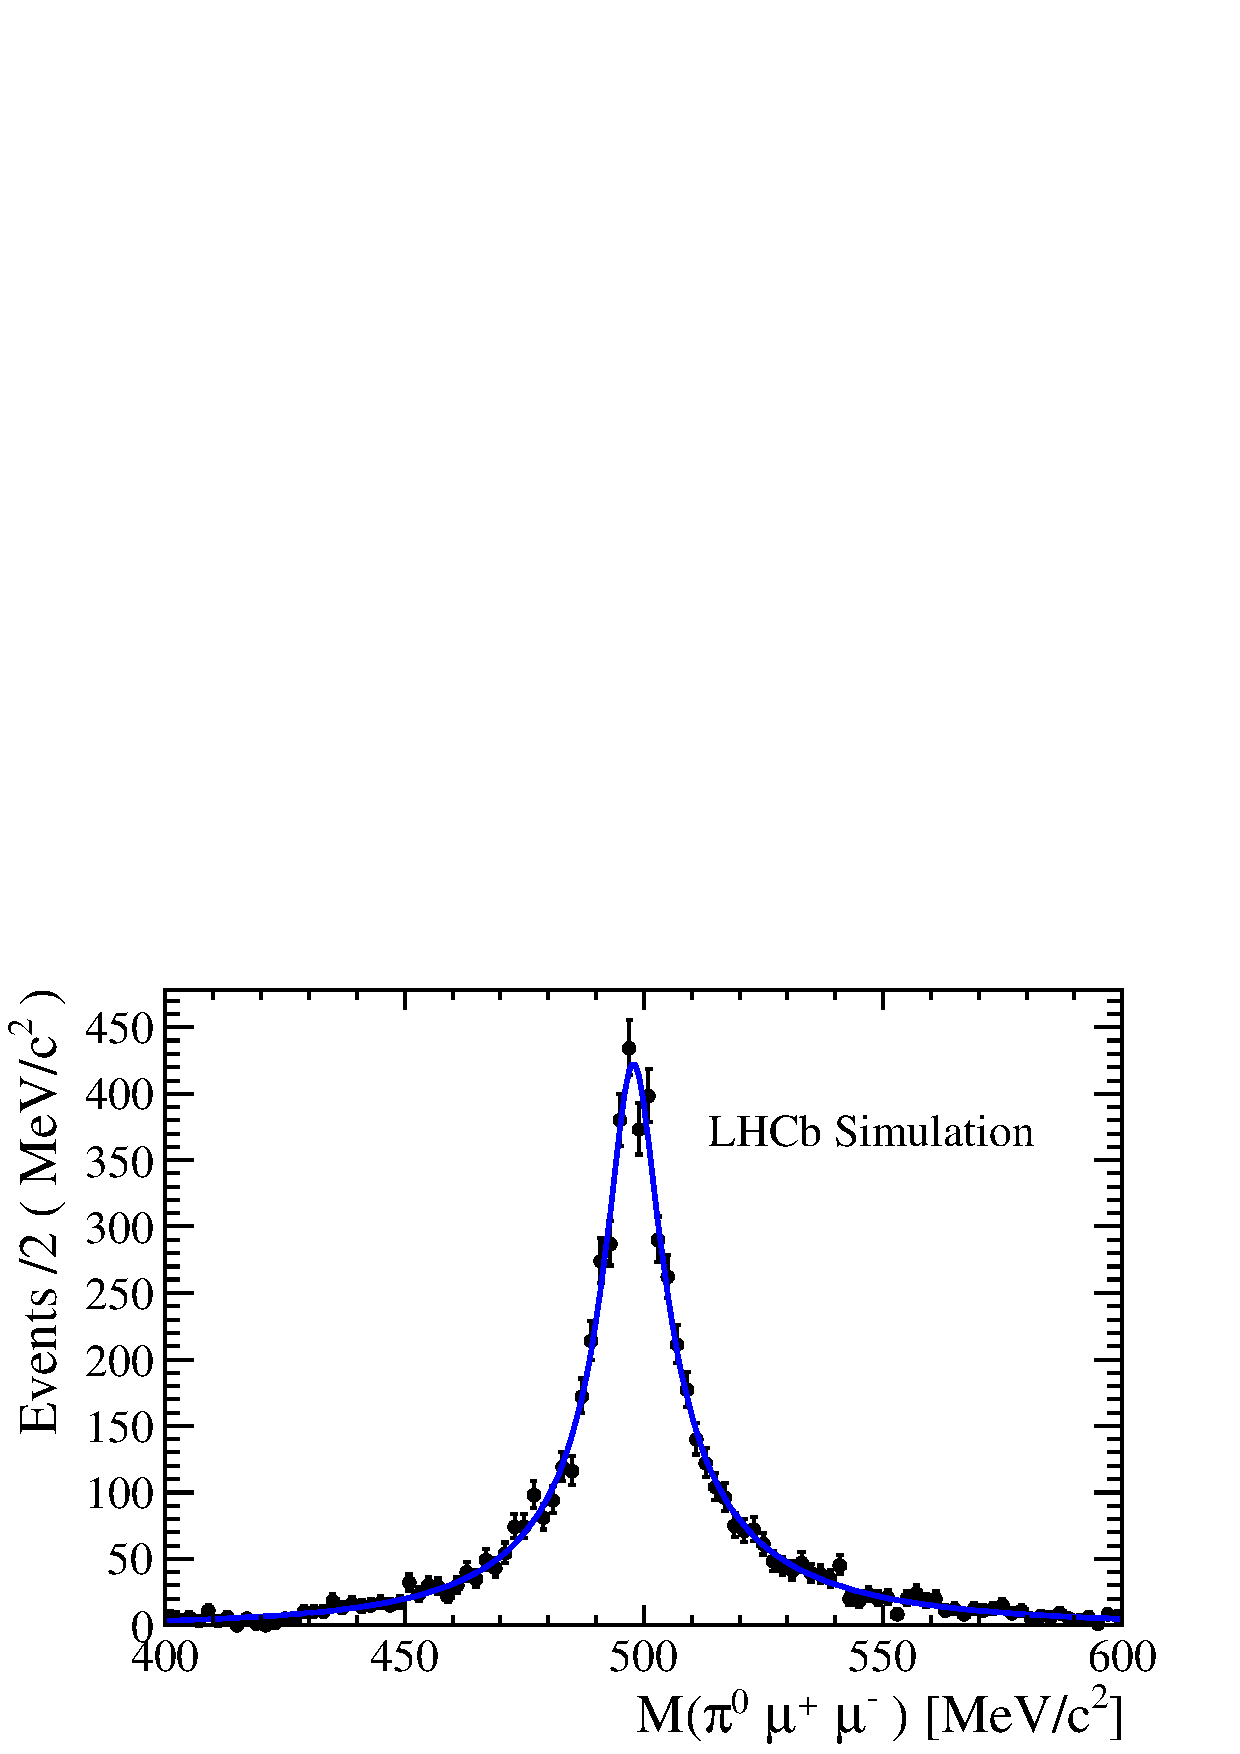
\includegraphics[width=0.49\textwidth]{Ipatia_pi0.pdf}
   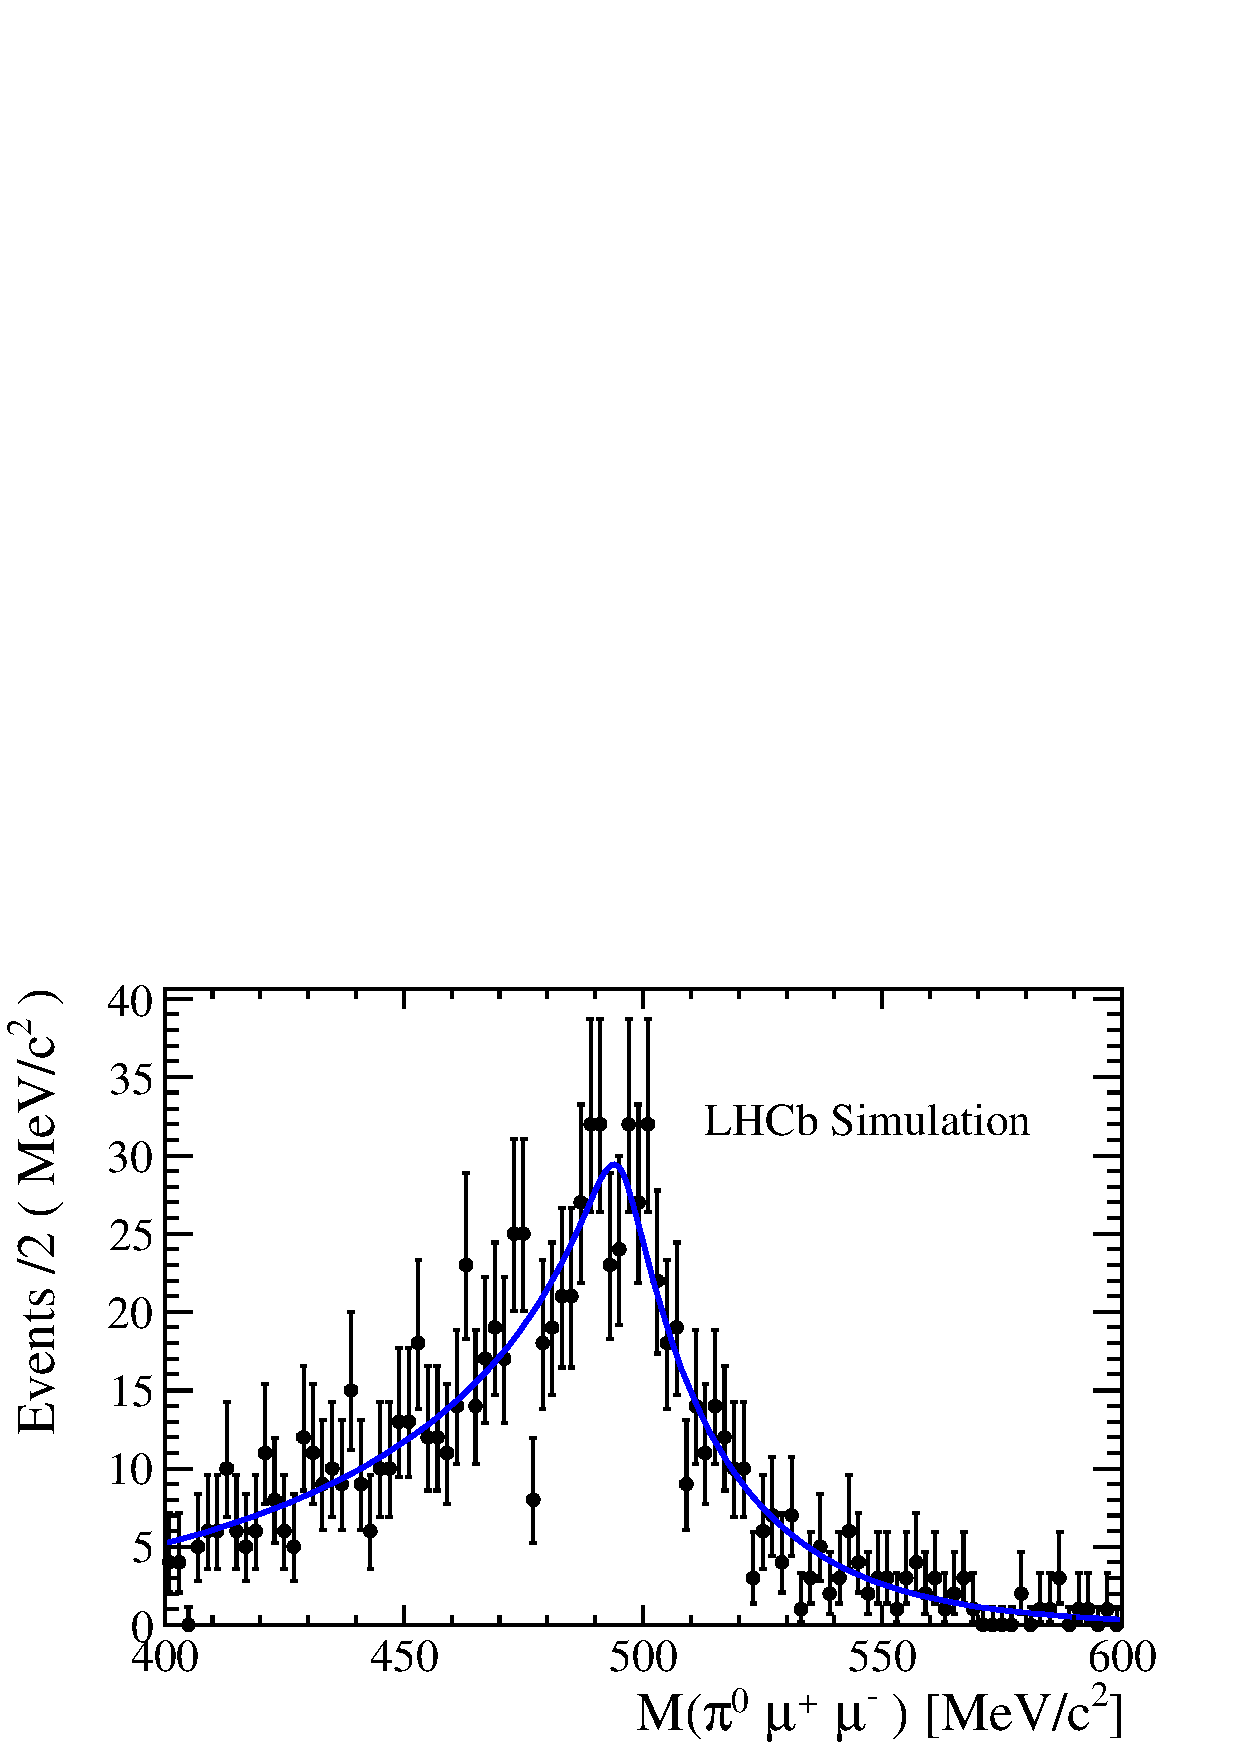
\includegraphics[width=0.49\textwidth]{Ipatia_nopi0.pdf}
\end{frame}


\begin{frame}{Background study}
 \textbf{$\PKz\to\APmuon\Pmuon\Pgamma\Pgamma$}
 \vspace{0.2cm}
 \begin{itemize}
  \setlength\itemsep{0.7em}
  \item ${\cal B}(\PKzL\to\APmuon\Pmuon\Pgamma\Pgamma) = 1^{+0.8}_{-0.6}\times 10^{-8}$
  \item[] $\rightarrow$ Reduced by the time acceptance by a factor of 0.001
  \item[] $\rightarrow$ Effectively, ${\cal B}_{LHCb}(\PKzL\to\APmuon\Pmuon\Pgamma\Pgamma) \approx {\cal O}(10^{-11})$ \\ \follows negligible
  \item ${\cal B}(\PKzS\to\APmuon\Pmuon\Pgamma\Pgamma)  =   \frac{{\cal B}(\PKzS\to\Pgamma\Pgamma)}{{\cal B}(\PKzL\to\Pgamma\Pgamma)} {\cal B}(\PKzL\to\APmuon\Pmuon\Pgamma\Pgamma)\sim 4.81\times10^{-14}$
  \item[] \follows also negligible
 \end{itemize}
\end{frame}

\begin{frame}{Background study}
 \textbf{$\PKz\to\Pgpp\Pgpm$}
 \vspace{0.2cm}
 \begin{itemize}
  \item Both \Pgp misidentified as \Pmu, combined with a random \Pgpz
  \item Mass peaks outside of the signal region
  \item Only residual tails enter the signal region -- add to the combinatorial background
 \end{itemize}
 
 \vspace{0.3cm}
 
 \textbf{$X\to\Pgpz\Pgpp\Pgpm$, e.g. $\Peta\to3\Pgp$}
 \vspace{0.2cm}
 \begin{itemize}
  \item Data reconstructed using the pion mass hypothesis for the two muons
  \item No peaking structure observed in the signal region
 \end{itemize}
 
 \vspace{0.3cm}
 
  \centering
  \includegraphics[width=0.3\textwidth]{M_VC_pipi_hyp.pdf}\hspace{0.4cm}
  \includegraphics[width=0.3\textwidth]{M_V0_pipi_hyp.pdf}
\end{frame}

\begin{frame}{Background study}
   \textbf{$\PKz\to\Pgpz\Pgpp\Pgpm$}
 \vspace{0.2cm}
  \begin{itemize}
  \setlength\itemsep{0.7em}
    \item Studied with MC and data
    \item Peak shifted towards lower energies wrt signal
    \item No evidence of significant contribution neither from data
    nor from MC, but precise determination not possible with current data
  \end{itemize}
 
 \vspace{0.5cm}
 
 \begin{minipage}{0.64\textwidth}
  \begin{itemize}
  \setlength\itemsep{0.7em}
    \item No significant impact on the sensitivity
    \item Modelled with a Landau distribution
    \item FULL toy MC assuming $\SI{50}{\per\femto\barn}$
   \item[] Without $\PKzL\to3\Pgp$:
	  $\sigma_{\pm}= 5.5\times10^{-10}$
   \item[] With \hspace{0.45cm}$\PKzL\to3\Pgp$:
	  $\sigma_{-}= (5.3\pm 0.7)\times10^{-10}$\\
	  \hspace{2.62cm} $\sigma_{+}= (5.5\pm 0.8)\times10^{-10}$
  \end{itemize}
 \end{minipage}
 \begin{minipage}{0.35\textwidth}
   \centering
    \includegraphics[width=0.99\textwidth]{landau.pdf}
%     \includegraphics[width=0.99\textwidth]{K3pi_FULL.pdf}\hspace{0.2cm} 
    \put(-59.,49.){\footnotesize \textcolor{red}{$\PKzL\to\Pgpz\Pgpp\Pgpm$}}
    \put(-59.,40.){\footnotesize \textcolor{red}{FULL}}\\
    
%     \vspace{0.5cm}
%     
%     \includegraphics[width=0.99\textwidth]{mK3pi_PARTIALL.pdf}
%     \put(-60.,40.){\footnotesize \textcolor{red}{$\PKzL\to\Pgpz\Pgpp\Pgpm$}}
%     \put(-60.,30.){\footnotesize \textcolor{red}{PARTIAL}}
 \end{minipage}
%  \end{minipage}
\end{frame}

\begin{frame}{Fit to the data}
    \textbf{Main background: combinatorial}
    \begin{itemize}
      \item Random track combinations 
      \item Monotonic shape (exponential)
      \item Shape determined directly from the fit to the data
    \end{itemize}
    
    \vspace{0.5cm}
 
    \textbf{Fit}
    \begin{itemize}
    \setlength\itemsep{0.6em}
    \item Consider only events in BDT region [0.6,1.0]
    \item Fit to $M(\Pgpz\Pmuon\APmuon)$ in four BDT bins of 0.1 each
    \item[] $\rightarrow$ Signal: Ipatia distribution
    \item[] $\rightarrow$ Background: Exponential function, free in the fit to the data
    \end{itemize}  
\end{frame}

\begin{frame}{Fit result FULL}
  \begin{center}
     \textbf{Run I data ($\SI{3}{\per\femto\barn}$) FULL fit result}\\ 
     
    \vspace{0.2cm}
    
    \textbf{$N(\KsPizMuMu)= 0\pm 19$}\\%6\cdot10^{-4}
    
    \vspace{0.2cm}
    
      \includegraphics[width=0.8\textwidth]{fit_FULL.pdf}\\
%     \begin{itemize}	
%     \item[] $\rightarrow$ Signal: Ipatia distribution
%     \item[] $\rightarrow$ Background: Exponential function
%     \end{itemize}
    
  \end{center}
\end{frame}

\begin{frame}{Fit result FULL}
  \begin{center}
     \textbf{2016 data ($\SI{0.3}{\per\femto\barn}$) PARTIAL fit result}\\ 
     
    \vspace{0.2cm}
    
    \textbf{$N(\KsPizMuMu)=24^{+15}_{-14}$}\\
    
    \vspace{0.2cm}
     
      \includegraphics[width=0.8\textwidth]{fit_PARTIAL.pdf}\\
%     \begin{itemize}	
%     \item[] $\rightarrow$ Signal: Ipatia distribution
%     \item[] $\rightarrow$ Background: Exponential function
%     \end{itemize}
    
  \end{center}
\end{frame}

\begin{frame}{Sensitivity study}
 \begin{itemize}
   \setlength\itemsep{0.7em}
    \item \KsPipPim used as a normalisation channel
    \item \KsPipPim prescaled by a factor of 0.001
    \item Sensitivity obtained from pseudo-experiments
    \item[]$\rightarrow$ Signal model from MC, background model from fit to the current data
    \item[]$\rightarrow$ Background yield extrapolated from current result assuming no signal contribution
    \item[]$\rightarrow$ Extrapolating expected signal yield from
 \begin{equation*}
%   {\cal B}(\KsPizMuMu) = 0.001\cdot\frac{N(\KsPizMuMu)}{ N(\KsPipPim)}\cdot\frac{\epsilon(\KsPipPim)}{\epsilon(\KsPizMuMu)}\cdot{\cal B}(\KsPipPim)
  N_{\rm sig} = \frac{{\cal B}(\KsPizMuMu)}{{\cal B}(\KsPipPim)}\frac{\epsilon(\KsPizMuMu)}{\epsilon(\KsPipPim)} N(\KsPipPim)\frac{{\cal L}_{fut}}{{\cal L}_{eff}}
 \end{equation*} 
 \end{itemize}
\end{frame}

\begin{frame}{Sensitivity study}
 \begin{itemize}
   \setlength\itemsep{0.7em}
  \item[]$\rightarrow$ Extrapolating expected signal yield from
    \begin{equation*}
    %   {\cal B}(\KsPizMuMu) = 0.001\cdot\frac{N(\KsPizMuMu)}{ N(\KsPipPim)}\cdot\frac{\epsilon(\KsPipPim)}{\epsilon(\KsPizMuMu)}\cdot{\cal B}(\KsPipPim)
      N_{\rm sig} = \frac{{\cal B}(\KsPizMuMu)}{{\cal B}(\KsPipPim)}\frac{\epsilon(\KsPizMuMu)}{\epsilon(\KsPipPim)} N(\KsPipPim)\frac{{\cal L}_{fut}}{{\cal L}_{eff}}
    \end{equation*} 
   \item Aiming for a much more efficient trigger after the upgrade
   \item Currently taking TIS events (unbiased sample) -- efficiency much lower than after the upgrade
   \item[] $\Rightarrow$ Current luminosity is effectively smaller, scale according to
  \begin{equation*}
    {\cal L}_{eff} = \epsilon^{TIS}(\KsPipPim){\cal L}_{LHCb} 
  \end{equation*}
 \end{itemize}
\end{frame}

\begin{frame}{Sensitivity study}
  \centering
  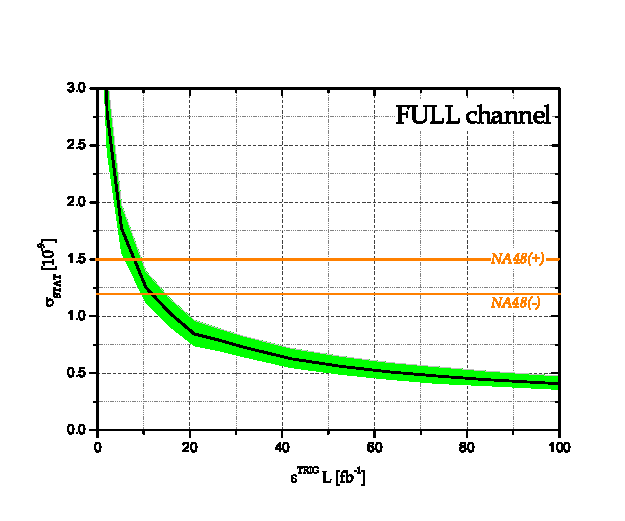
\includegraphics[width=0.49\textwidth]{sensit_FULL.pdf}
  \includegraphics[width=0.49\textwidth]{sensitPARTIAL.pdf}
  \begin{itemize}
      \item Good prospects for \KsPizMuMu given a high trigger efficiency ($>50\%$)
      \item FULL and PARTIAL sensitivity can be combined
  \end{itemize}
\end{frame}


\begin{frame}{Summary}
 \begin{itemize}
   \setlength\itemsep{0.7em}
  \item A precise knowledge of ${\cal B}(\KsPizMuMu)$ crucial for precise ${\cal B}(\PKzL\to\Pgpz\APmuon\Pmuon)$ SM prediction and BSM searches
  \item Sensitivity study of future LHCb sensitivity performed
  \item ${\cal B}(\KsPizMuMu)$ has good prospects at LHCb, sensitivity expected to be better than that of NA48 given a good strange particle trigger performance
%   \item PUB note ready
 \end{itemize}
 
 \vspace{0.5cm}
 
 \centering
 \Huge{Thank you for your attention!}
\end{frame}

\begin{frame}
 \centering
 \Huge{BACKUP}
\end{frame}

\begin{frame}{Stripping}
  \begin{table}
  \centering
  \footnotesize{
  \begin{tabular}{l@{\hspace{0.5cm}}l@{\hspace{0.5cm}}l@{\hspace{0.5cm}}l}
  \toprule
%    \textbf{Variables}                & $\PKzS\to\Pgpz\APmuon\Pmuon$ & $\PKzS\to\Pgpz\APmuon\Pmuon$ &$\PKzS\to\Pgpp\Pgpm$  \\
    \textbf{Variables}			    & {\bf FULL} &  {\bf PARTIAL} & $\PKzS\to\Pgpp\Pgpm$ \\
  \midrule
  Stripping line			  & K0s2Pi0MuMuLines & TriggerTestLine & K0s2Pi0MuMuLines\\
				    & & & RareNStrange\\
  Prescale			  & 1 & 1 & 0.001\\
  Input Particles              	  & StdAllLooseMuons & StdAllLooseMuons & StdNoPidsPions   \\
 				    & StdLooseResolvedPi0 & &   \\
   \PKzS  M                          & [400, 600] $\SI{}{\mega\eV}/c^{2}$  & - & [400, 600] $\SI{}{\mega\eV}/c^{2}$    \\
   $\mu^{+}\mu^{-}$  M               & -  & $<$ 450 $\SI{}{\mega\eV}/c^{2}$ &     \\
   \PKzS  tof                        & $>$ 0.06$\tau$ & $>$ 0.06$\tau$ & $>$ 0.1$\tau$  \\
   \PKzS  IP                         & $< 0.9$ \small mm &  - & $< 0.4$ \small mm    \\
   $\mu^{+}\mu^{-}$ DIRA             & $>$ 0 \small s & $>$ 0  \small s &  $>$ 0  \small s\\
   $\mu^{+}\mu^{-}$ DOCA            & $<$ 0.3 \small mm  & $<$ 0.1 \small mm  &  $<$ 0.3 \small mm     \\
   Daug. Track $\chi^{2}/ndof$   	  & $<$ 5 & $<$ 5 &  $<$ 5          \\
   Daug. IP$_{\chi^{2}}$         	  & $>$ 36 & $>$ 60 &  $>$ 100        \\
   Daug. ghost prob.        	  & - & $<$ 0.1 &  -        \\
   Daug. PID        	  	  & - & $>$ 0 &  -        \\
   Vertex $\rho$        	  	  & - & $>$ 4 \small mm&  -        \\
   Vertex $z$        	  	  & - & $>$ 650 \small mm &  -        \\
   Vertex $\chi^{2}/ndof$        	  	  & - & $<$ 9 &  -        \\
   $\delta_{z}$    		  & - & $>$ 0 \small mm &  -        \\
   $\cos\alpha$    		  & - & $>$ 0  &  -        \\
   IP$_{\text{max}}$/$\delta_{z}$    & - & $<$ 1/60 s$^{-1}$&  -        \\
  \bottomrule
  \end{tabular}
  }
  \end{table}
\end{frame}


\end{document}


\begin{frame}{MVA}
 \centering
 \textcolor{emerald}{\bf MVA training in three steps}\\
 
 \vspace{0.2cm}
 
  \textcolor{emerald}{{\bf Step 1} Continuous variables gaussianized, decorrelated and gaussianized again} \\
  
  \vspace{0.3cm}
 \begin{minipage}{0.45\textwidth}
    \begin{itemize}
     \setlength\itemsep{0.7em}
      \item $K_S^0$: IPs, $p_{T}$, vertex $\chi^{2}$, flight distance significance
      \item $\mu$: track fit $\chi^{2}$/NDF\textcolor{blue}{$^1$}, IPs, PID\textcolor{blue}{$^2$}, DOCA ($\mu^+\mu^-$)
      \item Angle between $\mu\mu$ and $\gamma\gamma$ planes (FULL only)
    \end{itemize}
    
  \begin{itemize}
  \setlength\itemsep{0.7em}
    \item $M(\gamma\gamma)$\textcolor{blue}{$^3$} (FULL only)
    \item Helicity angles (FULL only)
    \item SV coordinates\textcolor{blue}{$^4$} (suppress material interactions)
  \end{itemize}
 \end{minipage}
 \begin{minipage}{0.54\textwidth}
    
    \vspace{1cm}
%     \hspace{0.5cm} \textcolor{red}{---} signal \hspace{0.5cm} {---} background\\
    \includegraphics[width=0.49\textwidth]{mu1_track_Chi2DoFFULL.pdf}
      \put(-65,43){\textcolor{blue}{$1$}}
     \put(-25,42){\footnotesize{FULL}}
    \includegraphics[width=0.49\textwidth]{PIDmu1PARTIAL.pdf}
      \put(-65,43){\textcolor{blue}{$2$}}
      \put(-67,13){\footnotesize{PART.}}
      \put(-50,46){\footnotesize{\textcolor{red}{---} signal}
      \put(-27.5,-6){\footnotesize{{---} bkg}}}\\
    
    \includegraphics[width=0.49\textwidth]{pi0massFULL.pdf}
      \put(-65,43){\textcolor{blue}{$3$}}
      \put(-25,42){\footnotesize{FULL}}
    \includegraphics[width=0.49\textwidth]{SV3FULL.pdf}
      \put(-65,43){\textcolor{blue}{$4$}}
      \put(-25,42){\footnotesize{FULL}}
 \end{minipage}

\end{frame}



\begin{frame}{MVA}
 \begin{minipage}{0.65\textwidth}
  \textcolor{emerald}{{\bf Step 2} Output from Step 1 added into a common BDT with the discrete variables}
    \begin{itemize}
      \item Hits in: VELO$^{\textcolor{blue}{1}}$, TT, IT, OT
    \end{itemize}
  \textcolor{emerald}{{\bf Step 3} Flatten signal MVA response}
 \end{minipage}
 \begin{minipage}{0.34\textwidth}
  \includegraphics[width=0.99\textwidth]{mu1_hitsInVFULL.pdf}
      \put(-85,60){\textcolor{blue}{$1$}}
      \put(-60,55){\footnotesize{\textcolor{red}{---} signal}
      \put(-27.5,-6){\footnotesize{{---} background}}}
      \put(-25,22){\footnotesize{FULL}}\\
  \end{minipage}

 \hspace{1.5cm} {\bf BDT response FULL  \hspace{1cm} BDT response PARTIAL}\\
 \centering
 \includegraphics[width=0.35\textwidth]{BDT_sig_vs_bkg_FULL.pdf}\hspace{0.8cm}
 \includegraphics[width=0.35\textwidth]{BDT_sig_vs_bkg_PARTIAL.pdf}\\
 \vspace{0.1cm}
 \begin{itemize}
  \item Analysis performed in the BDT region [0.6, 1.0]
  \item[] Signal efficiency: \hspace{0.6cm} 40\% (FULL and PARTIAL)
  \item[] Background rejection: 99.3\% (FULL), 99.8\% (PARTIAL)
 \end{itemize}
\end{frame}
